\documentclass[12pt]{article} % Se vuoi scrivere in 14pt la classe dovrà essere 'extarticle'

% Pacchetti base
\usepackage[T1]{fontenc} % Codifica dei font: fornisce a LaTeX i caratteri accentati e altra roba di questo tipo
\usepackage[utf8]{inputenc} % Serve a LaTeX per interpretare correttamente i caratteri immessi nell'editor (utf8 oppure latin1)
\usepackage[greek.ancient,italian]{babel} % Lingue del documento, l'ultima è quella principale
\newcommand{\greco}{\foreignlanguage{greek}}
\addto\captionsitalian{\renewcommand{\abstractname}{Abstract}} % Per fare in modo che l'abstract venga nominato come "Abstract" e non come "Sommario"



% Formattazione generale
\usepackage{lmodern} % Il font usato sarà il Latin Modern (migliore nel posizionamento degli accenti rispetto a CModern)
\usepackage{helvet} % Pone l'Helvetica come font default per lo stile sans-serif
%\renewcommand{\familydefault}{\sfdefault} % Rende il sans-serif lo stile di default per il documento (eccetto che per la matematica)
\usepackage{microtype} % Pacchetto-boss per la microtipografia
\usepackage{indentfirst} % Produce il rientro della prima riga del primo capoverso di una sezione (Einaudi fa così XD)
%\setlength\parindent{0pt} % Elimina il rientro della prima riga di ogni capoverso
%\usepackage{layaureo} % Allarga un po' i margini rispetto allo standard, senza però allargarli troppo (discreta leggibilità) e mettendo larghezza e altezza del testo in sezione aurea
\usepackage{geometry} % Imposta i margini della pagina (continua riga sotto).
\geometry{a4paper,top=2cm,bottom=2cm,left=1.5cm,right=1.5cm,heightrounded} % Per aggiungere uno spazio di rilegatura piazzi alla fine 'bindingoffset= x mm'. Le dimensioni standard di Word sono 'top=2.5cm,bottom=2cm,left=2cm,right=2cm'. Per impostare tutte le pagine del documento in orizzontale inserisci anche l'opzione 'landscape'
\usepackage{enumitem} % Regola la spaziatura degli elenchi (continua sotto)
%\setlist{topsep=0.85em,parsep=0.45em,itemsep=0.1em} % 'topsep' regola la spaziatura fra i paragrafi prima e dopo l'ambiente, 'parsep' regola la spaziatura fra i paragrafi di uno stesso \item, 'itemsep' regola la spaziatura fra gli \item
\setdescription{labelindent=0em,labelsep=1em,leftmargin=\parindent} % 'labelindent' è la distanza del contrassegno dal margine della pagina, messa a 0 perché tutto il documento è un grande elenco quindi è inutile indentare | 'leftmargin' è l'indentazione delle righe successive alla prima in una voce, messa uguale a \parindent perché così è come se fosse un testo scritto normale | 'labelsep' è la distanza fra il contrassegno dal resto del testo nella prima riga di ogni voce

% Colori
\usepackage[svgnames,table,xcdraw]{xcolor} % Pacchetto che fornisce i colori, [svgnames] aumentare il database di colori disponibili
% Colori svgnames: Navy è più saturo di MidnightBlue
% \definecolor{jeans}{RGB}{0,42,84} % Definisce un colore che poi puoi usare altrove nel documento; prima il nome, poi il modello di colore (RGB è diverso da rgb) e poi la definizione del colore

% Figure e tabelle
\usepackage{graphicx} % Per inserire file esterni in figure
\usepackage{subfig} % Permette di inserire più figure all'interno dello stesso oggetto mobile
\usepackage{float} % Scrivendo [H] nelle preferenze di collocazione di un oggetto mobile, te lo mette proprio dove l'hai inserito.
\usepackage{wrapfig} % Per inserire figure "immerse" nel testo
\usepackage{booktabs} % Per produrre i filetti delle tabelle
\usepackage{caption} % Per produrre le didascalie (continua sotto)
\captionsetup{labelfont={sf,bf},tableposition=top,figureposition=bottom,font=small} % Specifiche per le didascalie: 'format=hang' allinea alla prima riga quelle successive | 'labelfont={sf,bf}' imposta l'etichetta della didascalia in caratteri senza grazie neri | specifica dove mettere la didascalia: sopra per le tabelle, sotto per le figure
\usepackage{floatflt,epsfig}
% Pacchetti scientifici
\usepackage[detect-all,output-decimal-marker={,},list-pair-separator={ e },list-final-separator={ e },range-units=single,range-phrase={--}]{siunitx} % Scrive correttamente le unità di misura SI: detect-all fa in modo che le unità di misura siano scritte riconoscendo le indicazioni di stile come grassetto e font serif/sans serif | output-decimal-marker specifica che il delimitatore decimale sia la virgola e non il punto | list-pair-separator specifica che il separatore fra due grandezze sia la 'e' | list-final-separator specifica che il separatore dell'grandezza sia la 'e' | range-phrase specifica il separatore fra la prima e la seconda grandezza | [retain-explicit-plus], che è meglio usare localmente, tiene esplicito il + di una grandezza
\usepackage{chemformula} % Per comporre formule chimiche
\usepackage{amsmath} % Pacchetto di estensioni per comporre la matematic
\usepackage{mathtools}
\usepackage{amssymb} % Rende disponibili una serie di simboli utili in matematica; carica automaticamente anche 'amsfonts'
% TikZ
\usepackage{tikz}
\usepackage{ulem}
\usepackage{boldline}
% Riquadri colorati tcolorbox
\usepackage{tcolorbox}
\newtcolorbox{riquadrostandard}[1]{colback=red!5!white,colframe=red!75!black,fonttitle=\bfseries,title=#1}
\newtcolorbox{regola}[1]{width=0.80\linewidth,colback=red!5,colframe=red!42,coltitle=black,halign title=center,fonttitle=\bfseries\large,title=#1}

% Bibliografia automatica
%\usepackage[hyperref=true,style=authoryear-comp]{biblatex} % Pacchetto per la bibliografia con le opzioni
%\addbibresource{Bibliografia-.bib} % Specifica da quale file prendere le referenze bibliografiche
% Altri pacchetti
\usepackage{footnotebackref} % Rende cliccabili le note a piè di pagina in modo che portino alla posizione nel testo a cui si riferiscono
\usepackage{pdfpages} % Per inserire pagine di un pdf esterno. Nel corpo del documento scrivi \includepdf[pages=2,3,5-8]{nome_pdf}; in base a dove metti il comando lui inizia una nuova pagina inserendo il pdf e quando ha finito riparte con una nuova pagina. Di default inserisce solo la pagina 1
\usepackage[font=small]{quoting} % Per inserire ambienti testuali come quello di abstract all'inizio; li invochi con i soliti \begin{quoting} ed \end{quoting}
\usepackage{comment} % Per inserire commenti lunghi
\usepackage{lipsum} % Genera testo fittizio
\hyphenation{} % Regola la sillabazione (se devi regolare più parole separale con uno spazio). Se vuoi regolare la sillabazione di una parola solo in un punto del documento, inserisci dentro \mbox{testo} ciò che non vuoi separare

% Nuovi comandi
\newcommand{\zariv}[1]{\colorbox{Yellow}{\textcolor{Magenta}{D@RiV}}}
\newcommand{\wariv}[1]{\colorbox{Yellow}{.}}
%\newcommand{nome_comando}[1]{come_deve_apparire} % Nuovo comando, insomma la cosa del libro di botanica. Con {nome_comando} assegni il nome che scriverai nel sorgente ogni volta che vuoi richiamare il comando, con {come_deve_apparire} dici cosa vuoi che LaTeX scriva ogni volta che piazzi il comando. Per esempio: \newcommand{\pianta}[1]{\textit{#1}}

% Interlinea
%\usepackage{setspace} % Regola l'interlinea, vedi sotto
%\singlespacing \onehalfspacing \doublespacing % Per interlinea 1, 1,5 e 2
%\renewcommand{\baselinestretch}{1.3} % Da usare solo per frontespizi o cose particolari! Aumenta la spaziatura di TUTTO, quindi usa solo per documenti ad una pagina e poco altro. Il valore 1.25 è CIRCA uguale a quello che ottieni con '\onehalfspacing'

% Spazio per pacchetti/comandi temporanei
\usepackage{multicol}
\usepackage{pdfpages}
% Altro
%\pdfminorversion='x' % Di default LaTeX produce un PDF versione 1.5, se vuoi fare in modo che produca versioni precedenti o successive sostituisci ad 'x' la seconda cifa della versione (per esempio 7 per PDF 1.7)
\overfullrule=3em % Stampa un quadrato nero accanto alle righe che sporgono dal margine in modo da segnalare che sono state composte male
\usepackage{hyperref} % Pacchetto-boss per i collegamenti ipertestuali e i metadati del pdf; caricalo per ultimo (ma prima di bookmarks)
\hypersetup{
	pdftitle={Esercitazione Idrodinamica Marco Falda },
	pdfauthor={Marco Falda},
	pdfsubject={ Idrodinamica },
	pdfkeywords={},
	colorlinks=true,
	linkcolor=MidnightBlue, % colore del collegamento \ref{} che porta all'elemento ipertestuale segnato con \label{}
	citecolor=Brown, % colore del collegamento \cite{} che porta all'elemento citato in bibliografia con \bibitem{}
	urlcolor=DarkRed, % colore del collegamento \url{} ad una pagina web
	% hidelinks % lo piazzi se vuoi che i collegamenti ipertestuali vengano neri come il testo normale
}
\usepackage{bookmark} % Produce l'indice nel pdf e permette di personalizzarlo meglio rispetto al solo hyperref

\begin{document}
	%\pagenumbering{gobble} % Per non non far comparire i numeri di pagina
	%\renewcommand{\abstractname}{\vspace{-\baselineskip}} % Se vuoi scrivere un abstract/sommario senza che ti esca la scritta abstract/sommario
	
\begin{comment}
NOTE
	- *pezza finché non trovo il modo di inserire gli accenti giusti da tastiera* : `` servono per fare le virgolette ALL'INIZIO DI PAROLA, '' servono per fare le virgolette ALLA FINE DI PAROLA
	oppure “”
	- La tilde ~, messa fra due parole senza spazio indica che non le si vuole separare da un "fine riga a capo". Però si accetta che possano essere separate dal trattino di sillabazione di fine riga
\end{comment}

% INSERIRE IL CODICE SOTTOSTANTE SUBITO DOPO \begin{document} NEL DOCUMENTO DELLA RELAZIONE

\thispagestyle{empty} % Per non non far comparire il numero di pagina
\newgeometry{top=2.5cm,bottom=2cm,left=1cm,right=1cm,heightrounded}
{\linespread{2.3}\selectfont
{\sffamily
	\begin{figure}
		\centering
		
\includegraphics[width=0.75\textwidth]{logounitrento2019.jpg}
	\end{figure}
		
	\vspace*{-1.5em}
		
	\begin{center}
		{\Large Corso di Laurea Magistrale}\\
		\vspace*{-0.8em}
		{\Large in Ingegneria per l'Ambiente e il Territorio}\\
		\vspace*{0.5em}
		{\Large A.A. 2019/2020}
				
		\vspace*{4em}
		
		{\Huge \textbf{Idrodinamica}}\\{\Large Esercitazione numerica I }
		
		\vspace*{4em}
		
		{\Large Prof. Dr. Marco Tubino}
	\end{center}
	
	\vspace*{3.2em}
	
	\begin{center}
	{\large
		Studenti:
	}
	{\large
		Marco Falda, Francesco Ghizzo
	}
	\end{center}

}
}
\restoregeometry

\newpage
\thispagestyle{empty}
\tableofcontents
\newpage
\listoffigures
\newpage

\section{Obiettivi}
\noindent Sviluppare un algoritmo per generare una stima della scala di deflusso a partire dalla geometria della sezione di un alveo, avvalendosi delle ipotesi del modello tridimensionale su bassa profondità e di moto stazionario e uniforme (equazione di Gauckler-Strickler) e utilizzando il metodo di Engelund. Individuare inoltre la profondità critica nella medesima sezione dell’alveo attraverso un metodo iterativo. Implementare l’algoritmo prodotto per mezzo di uno \textit{script} nel linguaggio Python e collaudare successivamente lo \textit{script} con i dati di geometria di sezioni complesse di alvei reali.

\newpage
\section{Introduzione}
\subsection{Scala di deflusso}
\noindent Nel contesto dello studio dei corsi d’acqua naturali vi è la necessità di reperire serie storiche di portata. La misura diretta, per mezzo, ad esempio, dell’integrazione spaziale del campo di velocità o di metodi globali, è purtroppo un processo caro, che richiede la presenza di un’equipe di tecnici qualificati e l’impiego di apparecchiature costose; è inoltre pericolosa nel caso di eventi estremi. 
Per queste ragioni si è storicamente fatto ricorso alla misura del pelo libero come \textit{proxy} della portata d’acqua, essendo gli idrometri strumenti economici e di facile lettura (Collischonn, 2013).
Al fine di poter mettere in relazione la lettura idrometrica con una stima di portata, si è creata la necessità della costruzione di scale di deflusso, ovvero curve empiriche, diverse da alveo ad alveo e da sezione a sezione, che assumono la forma di una legge di potenza: 

\begin{equation}
    Q=kY^m
    \label{eqn:scala_deflusso}
\end{equation}

\noindent Dove $Q$ [$m^3\cdot s^{-1}$]  rappresenta la portata, $Y$ [$m$] il tirante idraulico, ossia la differenza fra la quota della superficie libera e la quota del fondo, e $k$ ed $m$ [$adm]$ due coefficienti da stimare; $k$ ed $m$, tuttavia, non sono delle costanti. È possibile esplicitare $m$ derivando nell’equazione della scala di deflusso la portata per il tirante, ricavando così: 

\begin{equation}
    \frac{dQ}{dY}=mkY^{m-1}
    \label{eqn:m_1}
\end{equation}

\noindent Osservando che:

\begin{equation}
   kY^{m-1}=\frac{Q}{Y}
   \label{eqn:m_2}
\end{equation}

\noindent otteniamo:

\begin{equation}
    \frac{dQ}{dY}=m\frac{Q}{Y}
    \label{eqn:m_3}
\end{equation}

\noindent da cui si deduce che:

\begin{equation}
    m=\frac{dQ/dY}{Q/Y}
    \label{eqn:m_4}
\end{equation}

\noindent Sostituendo alla portata $Q$ l’equazione del moto uniforme di Gauckler-Strickler,
  
\begin{equation}
    U=ks\sqrt{iF}Rh^{\frac{2}{3}}
    \label{eqn:U_Gauckler-Strickler}
\end{equation}  
  
\begin{equation}
    Q=U\Omega=ks\sqrt{iF}Rh^{\frac{2}{3}}\Omega=ks\sqrt{iF}\Omega^{\frac{5}{3}}p^{-\frac{2}{3}}
    \label{eqn:Q_Gauckler-Strickler}
\end{equation}

\noindent (dove $U$ [$m\cdot s^{-1}$] è la velocità media della corrente, $\Omega$ [$m^2$] è l’area della sezione bagnata, $ks$ [$adm$] è un parametro, detto coefficiente di scabrezza di Strickler, che è inversamente proporzionale alla scabrezza del fondo, $R_h$ [$m$] è il raggio idraulico e $p$ [$m$] il perimetro bagnato) ricaviamo:

\begin{equation}
   m=\frac{dQ/dY}{Q/Y}=\frac{5}{3}\frac{d\Omega/dY}{\Omega/Y}-\frac{2}{3}\frac{dp/dY}{p/Y}
   \label{eqn:m_5}
\end{equation}

\noindent $m$ è pertanto funzione della geometria della sezione e del tirante idraulico. 
Il valore di $k$ racchiude invece la correlazione del flusso, oltre che con il raggio idraulico, con la pendenza e la scabrezza del fondo (Adami, 2019).

\subsection{\texorpdfstring{Coefficienti di Ragguaglio $\alpha$ e $\beta$}{} }

\noindent La potenza meccanica totale $W$ [$kg\cdot m^2\cdot s^{-3}$] di una corrente a superficie libera è data da un contributo fornito dall’energia potenziale:

\begin{equation}
   \int_{\Omega}^{}(\rho gh)ud\Omega
   \label{eqn:W_energia_potenziale}
\end{equation}

\noindent (dove $\rho$ [$Kg \cdot m^{-3}$] è la densità del fluido, $g$ [$m\cdot s^{-2}$] è l'accelerazione di gravità, $h$ [$m$] è la coordinata verticale della superficie libera e $u$ [$m\cdot s^{-1}$] è la velocità puntuale) e un contributo fornito dall’energia cinetica:

\begin{equation}
   \int_{\Omega}^{}\left(\frac{1}{2}\rho u^{2}\right)ud\Omega
   \label{eqn:W_energia_cinetica}
\end{equation}

\noindent Sommando entrambi i contributi:  

\begin{equation}
   W=\int_{\Omega}^{}(\rho gh+\frac{1}{2}\rho u^{2})ud\Omega=\rho gh\int_{\Omega}^{} ud\Omega + \frac{1}{2}\rho \int_{\Omega}^{} u^{3}d\Omega=\rho ghQ + \frac{1}{2}\rho \int_{\Omega}^{} u^{3}d\Omega
   \label{eqn:W}
\end{equation}

\noindent Il termine cinetico può inoltre essere riscritto come:

\begin{equation}
   \frac{1}{2}\rho \int_{\Omega}^{} u^{3}d\Omega=\frac{1}{2}\rho \alpha U^{3}\Omega
   \label{eqn:energia_cinetica_alfa}
\end{equation}

\noindent dove $\alpha$ [$adm$] è un coefficiente correttivo, detto coefficiente di ragguaglio dell’energia cinetica, ed esprime il rapporto fra l’energia cinetica di una corrente reale e l’energia che una corrente possederebbe se scorresse in un alveo di uguale sezione, ma con velocità uniforme e pari alla velocità media:

\begin{equation}
   \alpha=\frac{\frac{1}{2}\rho \int_{\Omega}^{} u^{3}d\Omega}{\frac{1}{2}\rho \alpha U^{3}\Omega}=\frac{\int_{\Omega}^{} u^{3}d\Omega}{U^{3}\Omega}=\frac{\frac{1}{\Omega}\int_{\Omega}^{} u^{3}d\Omega}{U^{3}}
   \label{eqn:alfa}
\end{equation}

\noindent In altre parole, il coefficiente $\alpha$ ci informa su quanto la velocità media di una corrente al cubo sia una buona approssimazione della media del campo di velocità reale elevato al cubo in ogni punto e integrato su tutta l’area.\\
La spinta meccanica totale di una corrente è anch’essa determinata da due componenti: una componente statica,

\begin{equation}
   \int_{\Omega}^{} Pd\Omega
   \label{eqn:S_comp_statica}
\end{equation}

\noindent che nasce dalla pressione $P$ [$m^2\cdot s^{-1}$] che agisce sulla sezione bagnata $\Omega$, e una componente dinamica, che rappresenta l’azione dinamica della quantità di moto:

\begin{equation}
   \int_{\Omega}^{} \rho u^{2}d\Omega
   \label{eqn:S_comp_dinamica}
\end{equation}

\noindent Sommando entrambe le componenti:   

\begin{equation}
   S=\int_{\Omega}^{} Pd\Omega+\int_{\Omega}^{} \rho u^{2}d\Omega=P\textsubscript{$G$}\Omega+\rho\int_{\Omega}^{} u^{2}d\Omega
   \label{eqn:S}
\end{equation}

\noindent La componente dinamica può essere anche resa nella forma:

\begin{equation}
    \rho\int_{\Omega}^{} u^{2}d\Omega=\rho\beta U^{2}\Omega
    \label{eqn:comp_dinamica_beta}
\end{equation}

\noindent dove $\beta$ [$adm$]è un coefficiente correttivo, detto coefficiente di ragguaglio della quantità di moto, e rappresenta il rapporto fra la quantità di moto effettiva della corrente e la quantità di moto di una corrente equivalente che attraversa la stessa sezione $\Omega$ e presenta velocità uniforme e pari alla velocità media della corrente $U$: 

\begin{equation}
   \beta=\frac{\rho \int_{\Omega}^{} u^{2}d\Omega}{\rho U^{2}\Omega}=\frac{\int_{\Omega}^{} u^{2}d\Omega}{U^{2}\Omega}=\frac{\frac{1}{\Omega}\int_{\Omega}^{} u^{2}d\Omega}{U^{2}}
   \label{eqn:beta}
\end{equation}

\noindent In altre parole, il coefficiente $\beta$ ci informa su quanto la velocità media di una corrente al quadrato sia una buona approssimazione della media del campo di velocità effettivo elevato al quadrato in ogni punto e integrato su tutta l’area.

\subsection{Carico Specifico e Profondità Critica}

\noindent Il carico specifico o energia specifica di una corrente in una sezione è definito come:

\begin{equation}
    E=H-z\textsubscript{$F$}=h+\alpha\frac{U^{2}}{2g}-z\textsubscript{$F$}=Y+\alpha\frac{U^{2}}{2g}=Y+\alpha\frac{Q^{2}}{2g\Omega^{2}}
    \label{eqn:E_1}
\end{equation}

\noindent dove $E$ [$m$] è un’energia per unità di peso, $H$ [$m$] è l’altezza della linea dell’energia e $z_F$ [$m$] è la coordinata verticale del fondo.
Considerato che $\Omega$ e $\alpha$ sono funzioni di $Y$ ed essendo $g$ costante, possiamo trattare $E$ come funzione delle sole variabili $Y$ e $Q$: $E=E(Y, Q)$.\\
Inoltre, poiché $\Omega$ è una funzione crescente con $Y$: 

\begin{equation}
    \lim_{Y\to\ 0} E|_{Q}=\lim_{Y\to\ 0} \left.\left(Y+\alpha\frac{Q^{2}}{2g\Omega^{2}}\right)\right|_{Q}=\lim_{Y\to\ 0} \left(\alpha \frac{Q^{2}}{2g\Omega^{2}}\right)= +\infty
    \label{eqn:E_2}
\end{equation}

\begin{equation}
    \lim_{Y\to\infty} E|_Q=\lim_{Y\to\infty} \left.\left(Y+\alpha\frac{Q^{2}}{2g\Omega^{2}}\right)\right|_Q=\lim_{Y\to\infty} (Y)= +\infty
    \label{eqn:E_3}
\end{equation}
Ne consegue che, imposto un valore di $Q$, deve esistere almeno un valore di tirante $Y$, detto critico ($Y\textsubscript{c}$) che corrisponde ad un minimo assoluto dell’energia specifica $E$.
Analiticamente, il minimo di $E$ a portata assegnata si ottiene imponendo:

\begin{equation}
    \left.\frac{\partial E}{\partial Y}\right|_Q=0
    \label{eqn:E_4}
\end{equation}

\noindent da cui:

\begin{equation}
    \left.\frac{\partial E}{\partial Y}\right|_Q=1+\frac{\alpha Q^2}{2g}\frac{\partial}{\partial Y}\left(\frac{1}{\Omega^{2}}\right)=1-\frac{\alpha Q^{2}}{g\Omega^{3}}\frac{\partial \Omega}{\partial Y}=0
    \label{eqn:E_5}
\end{equation}

\noindent Notando che la derivata della sezione per il tirante è, per definizione, la larghezza $B$,

\begin{equation}
    \frac{\partial \Omega}{\partial Y}=B(Y)
    \label{eqn:B}
\end{equation}

\noindent l’uguaglianza (\ref{eqn:E_5}) diventa:
\begin{equation}
    \left.\frac{\alpha Q^{2}B}{g\Omega^{3}}\right|_{Y=Y_{C}}=1
    \label{eqn:E_6}
\end{equation}

\noindent Infine, ricordando che il numero di Froude è definito come:

\begin{equation}
    Fr=\frac{U}{\sqrt{gY}}=\frac{U}{\sqrt{g\frac{\Omega}{B}}}=\frac{Q}{\Omega \sqrt{g\frac{\Omega}{B}}}
    \label{eqn:Froude}
\end{equation}

\noindent possiamo riscrivere (\ref{eqn:E_6}) come:

\begin{equation}
    \left.\frac{\alpha Q^{2}B}{g\Omega^{3}}\right|_{Y=Y_C}=\alpha \frac {Q^{2}}{\Omega^{2}}\left.\left(\frac{B}{g\Omega}\right)\right|_{Y=Y_C}=\alpha\left.\frac {Q^{2}}{\Omega^{2}\left(g\frac{\Omega}{B}\right)}\right|_{Y=Y_{C}}=\alpha Fr^{2}|_{Y=Y_C}=1
    \label{eqn:E_7}
\end{equation}

\noindent Assegnata quindi una portata $Q$, al fine di ottenere il tirante critico, dato che $\alpha$, $\Omega$ e $B$ sono funzioni di $Y$, basterà risolvere un’equazione implicita nella variabile $Y$:

\begin{equation}
    1-\alpha(Y)\frac{Q^{2}(Y)B(Y)}{g\Omega^{3}(Y)}=0
    \label{eqn:E_8}
\end{equation}
\noindent Data l'impossibilità di esplicitare Y, il suo valore potrà essere determinato soltanto mediante una soluzione numerica.

\newpage
\section{Metodologia}

\noindent La portata di generici corsi d’acqua può essere stimata assumendo valide le ipotesi: del modello tridimensionale su bassa profondità (ovvero moto planimetrico e con una direzione preferenziale), di stazionarietà e di uniformità. L’equazione analitica che si ricava a partire da queste ipotesi, come abbiamo visto, presenta la forma (\ref{eqn:Q_Gauckler-Strickler}), detta formula di Gauckler-Strickler.
In (\ref{eqn:Q_Gauckler-Strickler}), sia il valore del raggio idraulico $Rh$ che l’area della sezione $\Omega$ sono funzioni del tirante idraulico $Y$. Al fine di poter risolvere l’equazione è pertanto imprescindibile conoscere, per ogni $Y$, sia la forma che la dimensione della sezione bagnata. In contesti reali è tuttavia impossibile trovare un'espressione analitica che possa relazionare la geometria della sezione bagnata con il tirante della superficie libera $Y$, dal momento che il letto del fiume presenta una forma irregolare. L’eterogeneità nella composizione della sezione rende inoltre il valore della scabrezza del fondo non uniforme, con conseguente difficoltà nel quantificare il valore di $ks$. È evidente che l’unica strada possibile sia quella di ricorrere a metodi numerici.

\subsection{Metodo di Engelund}
\noindent Il metodo di Engelund è un metodo per la stima della portata d’acqua passante in una determinata sezione che presuppone, oltre alle ipotesi di bassa profondità e moto localmente uniforme previamente menzionate, tre ipotesi ulteriori, vale a dire:
\begin{itemize}
    \item La superficie libera rimane sempre orizzontale sulla sezione (la pendenza motrice non varia trasversalmente);
    \item La pendenza del fondo è costante sulla sezione;
    \item Il profilo di velocità che si sviluppa è logaritmico sulla verticale, ovvero, il tratto considerato ha una pendenza sufficientemente bassa da permettere di approssimare la normale al fondo con la verticale.
\end{itemize}

\subsection{Calcolo della portata}
\noindent Analiticamente, la portata passante per una sezione generica, se sono valide le premesse del modello su bassa profondità, è data dall’integrale della distribuzione della velocità $U$ sulla sezione $y = [0, B]$:

\begin{equation}
    Q=\int_{\Omega}^{} ud\Omega=\int_{0}^{B}UYdy=\sqrt{iF}\int_{0}^{B}ksRh^{\frac{2}{3}}Ydy
    \label{eqn:Q_Engelund_1}
\end{equation}

\noindent dove $B$ è la larghezza della sezione [$m$] e dove la velocità U è una funzione puramente della coordinata orizzontale $y$ (la velocità è infatti mediata sulla verticale).
Dal momento che l’operatore integrale gode della proprietà additiva, la portata nell’equazione (\ref{eqn:Q_Engelund_1}) può essere espressa come:

\begin{equation}
    Q=\sum_i^n Q_i
    \label{eqn:Q_Engelund_2}
\end{equation}

\noindent dove $Q\textsubscript{i}$ è uguale a:

\begin{equation}
    Q\textsubscript{i}=\sqrt{iF}\int_{0}^{h} ks(y)Rh^{\frac{2}{3}}(y)Y(y)dy
    \label{eqn:Q_Engelund_3}
\end{equation}

\noindent In altre parole, il metodo di Engelund si basa sul semplice presupposto che la portata totale è equivalente alla sommatoria della portata passante per la sezione di ciascuno degli $n$ sotto-intervalli di larghezza $h$. La procedura prevede quindi innanzitutto la suddivisione trasversale dell’alveo in intervalli regolari, ai quali si assegnano ciascuno un valore di tirante e di scabrezza e per ognuno dei quali sarà necessario risolvere, attraverso opportuni metodi numerici, l’integrale dell’equazione (\ref{eqn:Q_Engelund_3}).

\noindent Poiché la geometria degli intervalli è conosciuta, essendo quella di un trapezio, possiamo cercare un’espressione analitica per il raggio idraulico. Il raggio idraulico è dato dal rapporto:

\begin{equation}
    R\textsubscript{h}=\frac{\Omega}{p}
    \label{eqn:Rh_1}
\end{equation}


\noindent che per un trapezio infinitesimo di altezza $dy$ e base minore e maggiore di lunghezza rispettivamente $Y$ e $Y+dY$ (Figura \ref{fig:Rh locale}) vale:

\begin{equation}
    R\textsubscript{h}=\frac{d\Omega}{dp}
    \label{eqn:Rh_2}
\end{equation}

\noindent dove l'area infinitesima $d\Omega$ è uguale a:

\begin{equation}
    d\Omega=\frac{(Y+(Y+dY))dy}{2}
    \label{eqn:dOmega}
\end{equation}

\begin{figure}
    \centering
    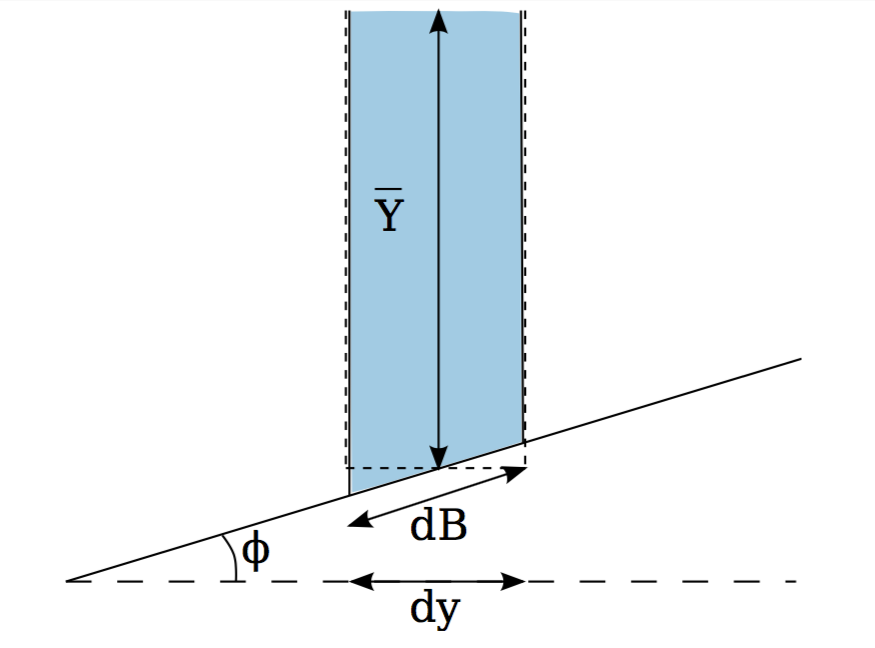
\includegraphics[width=0.4\textwidth]{Rh locale.png}
    \caption{Raggio idraulico locale}
    \label{fig:Rh locale}
\end{figure}

\noindent e il perimetro bagnato $dp$ vale a sua volta:

\begin{equation}
    dp=\frac{dy}{cos\phi}
    \label{eqn:dp}
\end{equation}

\noindent dove $\phi$ rappresenta l’angolo tra l’orizzontale e il fondo dell’alveo. Sostituendo $d\Omega$ (\ref{eqn:dOmega}) e $dp$ (\ref{eqn:dp}) nella definizione di $Rh$ (\ref{eqn:Rh_2}) e sviluppando otteniamo:

\begin{equation}
    R\textsubscript{h}=\frac{d\Omega}{dp}=\frac{(2Ydy+dYdy)/2}{dy/cos\phi}
    \label{eqn:Rh_3}
\end{equation}

\noindent e a meno di infinitesimi di ordine superiore:

\begin{equation}
    R\textsubscript{h}=\frac{d\Omega}{dp}=\frac{2Ydy/2}{dy/cos\phi}=\frac{Ydy}{dy/cos\phi}=Ycos\phi
    \label{eqn:Rh_4}
\end{equation}

\noindent Ci è dunque possibile rielaborare l’equazione (\ref{eqn:Q_Engelund_3}) esprimendo l’integrale come funzione soltanto del coefficiente di Strickler $ks$, del coseno di $\phi$ e del tirante idraulico $Y$:

\begin{equation}
    Q\textsubscript{i}=\sqrt{iF}\int_{0}^{h} ks(y)cos\phi^{\frac{2}{3}}(y)Y^{\frac{5}{3}}(y)dy
    \label{eqn:Q_Engelund_4}
\end{equation}

\begin{equation}
   Q=\sum_i^n Q\textsubscript{i}=\sqrt{iF}\int_{0}^{B} ks(y)cos\phi^{\frac{2}{3}}(y)Y^{\frac{5}{3}}(y)dy
    \label{eqn:Q_Engelund_5}
\end{equation}

\subsection{\texorpdfstring{Coefficiente di ragguaglio dell’Energia Cinetica $\alpha$}{}}

\noindent Mediando la definizione di $\alpha$ (\ref{eqn:alfa}) sulla verticale:

\begin{equation}
    \alpha=\frac{\int_{\Omega}^{} u^{3}d\Omega}{U^{3}\Omega}=\frac{\int_{0}^{B} u^{3}(y)Y(y)dy}{U^{2}Q}=\frac{\Omega^{2}}{Q^{3}}\int_{0}^{B}u^{3}(y)Y(y)dy
    \label{eqn:alfa_Engelund_1}
\end{equation}

\noindent Sostituendo alla velocità $u$ la formula di Gauckler-Strickler per il moto uniforme (\ref{eqn:U_Gauckler-Strickler}) e alla portata $Q$ l’espressione a cui siamo pervenuti mediando sulla profondità (\ref{eqn:Q_Engelund_5}) e avvalendoci della stessa formulazione del raggio idraulico ricavata in (\ref{eqn:Rh_4}):
\begin{equation}
    \begin{gathered}
        \alpha=\Omega^{2}\frac{\int_{0}^{B}\left(ks\sqrt{iF}Rh^{\frac{2}{3}}\right)^{3}Y(y)dy}{[\sqrt{iF}\int_{0}^{B} ks(y)cos\phi^{\frac{2}{3}}(y)Y^{\frac{5}{3}}(y)dy]^{3}}
        \\
        \alpha=\Omega^{2}\frac{\int_{0}^{B}\left(ks(Ycos\phi)^{\frac{2}{3}}\right)^{3}Y(y)dy}{[\int_{0}^{B} ks(y)cos\phi^{\frac{2}{3}}(y)Y^{\frac{5}{3}}(y)dy]^{3}}
        \\
        \alpha=\Omega^{2}\frac{\int_{0}^{B}ks^3(y)cos\phi^{2}(y)Y^{3}(y)dy}{[\int_{0}^{B} ks(y)cos\phi^{\frac{2}{3}}(y)Y^{\frac{5}{3}}(y)dy]^{3}}
    \end{gathered}
    \label{eqn:alfa_Engelund_2}
\end{equation}

\subsection{\texorpdfstring{Coefficiente di ragguaglio della Quantità di Moto $\beta$}{}}

\noindent Mediando la definizione di beta (\ref{eqn:beta}) sulla verticale:

\begin{equation}
   \beta=\frac{\int_{\Omega}^{} u^{2}d\Omega}{ U^{2}\Omega}=\frac{\int_{0}^{B} u^{3}(y)Y(y)dy}{UQ}=\frac{\Omega \int_{0}^{B} u^{3}(y)Y(y)dy}{Q^{2}}
   \label{eqn:beta_Engelund_1}
\end{equation}

\noindent Sostituendo alla velocità $u$ la formula di Gauckler-Strickler per il moto uniforme (\ref{eqn:U_Gauckler-Strickler}) e alla portata $Q$ l’espressione a cui siamo pervenuti mediando sulla profondità (\ref{eqn:Q_Engelund_5}) e avvalendoci della stessa formulazione del raggio idraulico ricavata in (\ref{eqn:Rh_4}):

\begin{equation}
    \begin{gathered}
        \beta=\Omega^{2}\frac{\int_{0}^{B}(ks\sqrt{iF}Rh^{\frac{2}{3}})^{2}Y(y)dy}{[\sqrt{iF}\int_{0}^{B} ks(y)cos\phi^{\frac{2}{3}}(y)Y^{\frac{5}{3}}(y)dy]^{2}}
        \\
        \beta=\Omega^{2}\frac{\int_{0}^{B}(ks(Ycos\phi^{\frac{2}{3}}))^{2}Y(y)dy}{[\int_{0}^{B} ks(y)cos\phi^{\frac{2}{3}}(y)Y^{\frac{5}{3}}(y)dy]^{2}}
        \\
        \beta=\Omega^{2}\frac{\int_{0}^{B}ks^{2}(y)cos\phi^{\frac{4}{3}}(y)Y^{\frac{7}{3}}(y)dy}{[\int_{0}^{B} ks(y)cos\phi^{\frac{2}{3}}(y)Y^{\frac{5}{3}}(y)dy]^{2}}
        \end{gathered}
        \label{eqn:beta_Engelund_2}
\end{equation}

\subsection{Metodo dei trapezi}

\noindent Il metodo dei trapezi è una tecnica per la risoluzione di integrali definiti tramite la discretizzazione del dominio della funzione integranda in intervalli di larghezza costante. Il metodo si basa sull’ipotesi che la media dei valori che la funzione assume agli estremi di un intervallo sia una buona approssimazione del valor medio di tutti i valori che la funzione assume dentro l’intervallo; in altre parole, si presume che, in ogni tratto in cui si è suddiviso il dominio, se il numero dei tratti è sufficientemente alto, la funzione sia rappresentabile per mezzo di una retta. La procedura prevede il calcolo delle aree dei trapezi contenuti in ogni intervallo, la somma delle quali fornisce un valore approssimato dell’integrale totale; l'accuratezza di questa approssimazione dipende dal numero di intervalli di discretizzazione.

\noindent In formule:

\begin{equation}
    \int_{x_1}^{x_2} f(x)dx\approx\frac{f(x\textsubscript{1})+f(x\textsubscript{2})}{2}(x\textsubscript{2}-x\textsubscript{1})
    \label{metodo_trapezi}
\end{equation}

\noindent Applicando il metodo dei trapezi a (\ref{eqn:Q_Engelund_4}), possiamo ottenere una formula operativa per il calcolo della portata grazie al metodo di Engelund:

\begin{equation}
    Q\textsubscript{i}\approx\sqrt{iF}cos\phi^{\frac{2}{3}}\textsubscript{i,i+1}\frac{(ks\textsubscript{i}Y_i^{\frac{5}{3}}+ks\textsubscript{i+1}Y_{i+1}^{\frac{5}{3}})}{2}(y\textsubscript{i+1}-y\textsubscript{i})
    \label{eqn:Q_trapezi_1}
\end{equation}

\noindent La (\ref{eqn:Q_Engelund_5}) diventa pertanto:

\begin{equation}
    Q\approx\sqrt{iF}\sum_{i=1}^n cos\phi^{\frac{2}{3}}\textsubscript{i,i+1}\frac{(ks\textsubscript{i}Y_i^{\frac{5}{3}}+ks\textsubscript{i+1}Y_{i+1}^{\frac{5}{3}})}{2}(y\textsubscript{i+1}-y\textsubscript{i})
    \label{eqn:Q_trapezi_2}
\end{equation}

\noindent dove $cos\phi_{i,i+1}$ è uguale a (Figura \ref{fig:suddivisione_alveo}):

\begin{equation}
    cos\phi_{i,i+1} = \frac{dy}{dB} = \frac{y_{i+1}-y_{i}}{\sqrt{(y_{i+1}-y_{i})^2+(z_{i+1}-z_{i})^2}}
\end{equation}

\begin{figure}
    \centering
    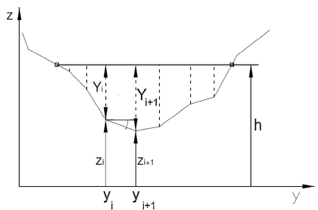
\includegraphics[scale=1.3]{suddivisione alveo.png}
    \caption{$cos\phi_{i,i+1}$ per un generico intervallo $i,i+1$}
    \label{fig:suddivisione_alveo}
\end{figure}

\subsection{Metodo della quadratura di Gauss}

\noindent Il metodo dei trapezi è intuitivo e di facile comprensione; ciononostante, non è molto efficiente e può richiedere una fitta discretizzazione e, di conseguenza, un grande numero di cicli da parte del calcolatore per ottenere risultati di precisione accettabile. 
Il metodo dei trapezi è, d’altronde, soltanto un caso specifico, in cui gli intervalli sono imposti regolari ed equidistanti tra loro, in una famiglia di metodi di integrazione numerica, detti di quadratura. I metodi di quadratura stimano il valore dell’integrale di una funzione come la sommatoria del valore che la funzione assume in determinati punti discreti, detti nodi, moltiplicato per un peso $\omega_{j}$ (Quarteroni et al., 2014):

\begin{equation}
    \int_{x_1}^{x_2} f(x)dx\approx\sum_{j=1}^n f(x_j)\omega_j
    \label{eqn:formule_quadratura}
\end{equation}

\noindent Il metodo della quadratura di Gauss, in particolare, si prefigge l’obiettivo, dato un numero di nodi $n$, di ottimizzare sia la posizione dei nodi che il valore dei pesi, affinché l’accuratezza sia la maggiore possibile, ovvero affinché sia minimizzato lo scarto fra il valore analitico e numerico dell’integrale definito. Per ragioni che esulano dallo scopo di questo studio, è possibile dimostrare che la posizione ottimale dei nodi si ha in prossimità delle radici di un polinomio ortogonale. 
La formula generale della quadratura di Gauss, definita nell’intervallo $[-1,1]$, è la seguente:

\begin{equation}
    \int_{-1}^{1} f(\xi)d\xi\approx\sum_{j=1}^{n_G} f(\xi_{j})\omega_{j}
    \label{eqn:Gauss-Legendre_1}
\end{equation}

\noindent dove $n_G$ è il numeri di nodi adottati, le ascisse $\xi_{j}$ sono le radici del polinomio di Legendre di ordine $n_G$ (quadratura di Gauss-Legendre) e i pesi $\omega_j$ sono calcolati risolvendo il seguente sistema di equazioni:
\begin{align}
    \sum_{j=1}^{n_G} \omega_j L_i(\xi_j) = \begin{cases}\textrm{2 \textit{se i} = 0}\\\textrm{0 \textit{altrimenti}}\end{cases} && i = 0, 1, ... n-1
    \label{eqn:pesi_Gauss-Legendre_1}
\end{align}

\noindent In notazione matriciale:
\begin{equation}
    \begin{vmatrix} & & & &  & &\\ & & & & & & \\ & & &L_i(\xi_j)& &  &\\ & & & & & &\\ & & & & & & \end{vmatrix}\cdot\begin{vmatrix}\\\\\omega_j\\\\\\\end{vmatrix}=\begin{vmatrix}2\\0\\...\\...\\0\end{vmatrix}
    \label{eqn:pesi_Gauss-Legendre_2}
\end{equation}

\noindent Gli zeri $\xi_j$ dei polinomi di Legendre di ordine $n$ ($L_n$) e i corrispettivi pesi $\omega_j$ calcolati risolvendo il sistema (\ref{eqn:pesi_Gauss-Legendre_2}) sono presentati in Tabella (\ref{tab:Legendre}) sino ad $n = 4$. 

\begin{table}[h]
    \centering
    \begin{tabular}{cccc}
        $n$ &$\xi_j$ &$\omega_j$ &$L_n$\\
        \hlineB{3}
        $0$ & $-$ & $-$ & $1$\\\hline
        $1$ & $0$ & $2$ & $x$\\\hline
        $2$ & $\pm\frac{1}{\sqrt{3}}$  & $1$ & $x^2-\frac{1}{3}$\\\hline
        $3$ & $0$ & $\frac{8}{9}$ & $x^3-\frac{3}{5}x$\\
            & $\pm\sqrt{\frac{3}{5}}$ & $\frac{5}{9}$\\\hline
        $4$ & $\pm\sqrt{\frac{3}{7}}$ & $\frac{18+\sqrt{30}}{36}$ & $x^4-\frac{6}{7}x^2+\frac{3}{35}$\\
            & $\pm\sqrt{\frac{3}{7}}$ & $\frac{18-\sqrt{30}}{36}$\\\hline
\end{tabular}
    \caption{Polinomi di Legendre di ordine $n$ ($Ln$), i rispettivi zeri $\xi_j$ e i pesi $\omega_j$}
    \label{tab:Legendre}
\end{table}

\noindent Estendendo la formula (\ref{eqn:Gauss-Legendre_1}) ad un generico intervallo $[x_1,x_2]$:

\begin{equation}
    \int_{x_1}^{x_2} f(x)dx\approx\left(\frac{x\textsubscript{2}-x\textsubscript{1}}{2}\right)\sum_{j=1}^{n_G} \omega_j f\left(\frac{x\textsubscript{2}-x\textsubscript{1}}{2}x_{G,j}+\frac{x\textsubscript{2}+x\textsubscript{1}}{2}\right)
    \label{eqn:Gauss-Legendre_2}
\end{equation}

\noindent che applicata a (\ref{eqn:Q_Engelund_4}) diventa:

\begin{equation}
    Q\textsubscript{i}\approx\sqrt{iF}cos\phi^{\frac{2}{3}}\textsubscript{i,i+1}\left(\frac{y\textsubscript{i+1}-y\textsubscript{i}}{2}\right)\sum_{j=1}^{n_G} \omega\textsubscript{j}\hat{ks}\textsubscript{j}\hat{Y}\textsubscript{j}^{\frac{5}{3}}
    \label{eqn:Q_Gauss-Legendre_1}
\end{equation}

\noindent dove $\hat{ks}\textsubscript{j}$ e $\hat{Y}\textsubscript{j}$ sono i valori che le funzioni $ks(y)$ e $Y(y)$ assumono nelle coordinate suggerite dal metodo della quadratura di Gauss esteso ad un intervallo generico $[y\textsubscript{i}, y\textsubscript{i+1}]$: 

\begin{equation}
    \hat{ks}_{j}=ks\left(\frac{y_{i+1}-y_{i}}{2}x_{G,j}+\frac{y_{i+1}+y_{i}}{2}\right)
\end{equation}

\begin{equation}
    \hat{Y}_{j}=Y\left(\frac{y_{i+1}-y_{i}}{2}x_{G,j}+\frac{y_{i+1}+y_{i}}{2}\right)
\end{equation}

\noindent Ammettendo che le funzioni $ks(y)$ e $Y(y)$ possano essere approssimate linearmente nell’intervallo $[y\textsubscript{i}, y\textsubscript{i+1}]$:

\begin{equation}
    \hat{ks}_{j}=ks\left(\frac{y_{i+1}-y_{i}}{2}x_{G,i}+\frac{y_{i+1}+y_{i}}{2}\right)\approx\frac{ks_{i+1}-ks_{i}}{2}x_{G,j}+\frac{ks_{i+1}+ks_{i}}{2}
\end{equation}

\begin{equation}
    \hat{Y}_{j}=Y\left(\frac{y_{i+1}-y_{i}}{2}x_{G,i}+\frac{y_{i+1}+y_{i}}{2}\right)\approx\frac{Y\textsubscript{i+1}-Y{i}}{2}x\textsubscript{G,j}+\frac{Y\textsubscript{i+1}+Y{i}}{2}
\end{equation}

\noindent Sommando tutti i contributi otteniamo finalmente:

\begin{equation}
    Q\approx\sqrt{i_F}\sum_{i=1}^n\left(cos\phi^{\frac{2}{3}}\textsubscript{i,i+1}\frac{y\textsubscript{i+1}-y\textsubscript{i}}{2}\sum_{j=1}^{n_G}\omega\textsubscript{j}\hat{ks}\textsubscript{j}\hat{Y}\textsubscript{j}^{\frac{3}{5}}\right)
    \label{eqn:Q_Gauss-Legendre_2}
\end{equation}

\subsection{Metodo della bisezione}

\noindent Il metodo della bisezione si basa su una proprietà delle funzioni continue, detta teorema degli zeri per le funzioni continue (Quarteroni et al., 2014):
\begin{quote}
“data una funzione $f$ definita e continua in un intervallo $[a,b] \in D$, se $f(a) f(b)  < 0$, ovvero se  $f(a)$ ed $f(b)$ hanno segni discordi, allora esisterà sempre un punto $c \in ]a,b[$ tale che $f(c) = 0$; in altre parole, esisterà sempre almeno un punto in cui la funzione si annulla dentro l’intervallo.”
\end{quote}

\begin{figure} [H]
    \centering
    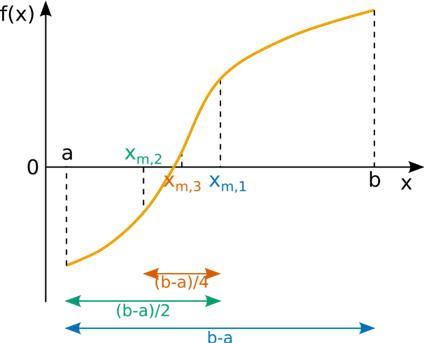
\includegraphics[scale=0.9]{bisezione.png}
    \caption{Metodo della bisezione}
    \label{fig:bisezione}
\end{figure}

\noindent Operativamente, una volta individuato un intervallo $[a,b]$ i cui estremi $a$ e $b$ soddisfino le condizioni imposte dal teorema degli zeri per le funzioni continue, possiamo ulteriormente suddividerlo in due sotto-intervalli $[a,x_m]$ e $[x_m,b]$ (dove $x_m$ rappresenta la coordinata del punto medio dell’ intervallo $[a,b]$) e controllare quale dei due continui a rispettare le condizioni del teorema. Questa strategia, detta di bisezione (Figura \ref{fig:bisezione}), si ripete iterativamente e si arresta al passo in corrispondenza del quale si abbia $|x_m - c| \leq \epsilon$, dove $\epsilon$ rappresenta una precisione scelta a piacere.

\subsection{Implementazione}

\noindent L’algoritmo è stato tradotto nel linguaggio di programmazione Python. All’interno del programma, i parametri forniti dall’utente sono il file contenente i dati di geometria dell’alveo, il numero di punti di discretizzazione verticale e il numero massimo di iterazioni nel calcolo della profondità critica, oltre alla pendenza del fondo $i_F$.
L'algoritmo simula tanti valori di superficie libera quanti sono i punti di discretizzazione verticale. Ad ogni iterazione, stabilita una quota $h$, a partire dai dati di geometria dell’alveo viene calcolata l’area della sezione $\Omega$, la larghezza del profilo di corrente $B$, la portata defluente in condizioni di moto uniforme $Q$ e i coefficienti di ragguaglio $\alpha$ e $\beta$. 
Innanzitutto è identificata la sezione bagnata: sottraendo punto a punto, lungo la direzione orizzontale, la quota del fondo $z_F(y)$ alla quota del pelo libero $h(y)$ è prodotto un array dei valori di tirante $Y(y)$. È possibile in questo modo individuare quali siano i punti interessati dalla corrente e quali siano i punti ad una quota maggiore del pelo libero, che possono essere perciò esclusi dall’analisi, e valutare così facilmente $\Omega$ e $B$. In seguito vengono chiamate delle apposite funzioni che calcolano la portata passante $Q$ (\ref{eqn:Q_Engelund_5}) e i coefficienti di ragguaglio $\alpha$ (\ref{eqn:alfa_Engelund_2}) e $\beta$ (\ref{eqn:beta_Engelund_2}), avvalendosi sia del metodo dei trapezi (\ref{eqn:Q_trapezi_2}), che della quadratura gaussiana (\ref{eqn:Q_Gauss-Legendre_2}) con 2, 3 e 4 nodi. 
Come ultimo passaggio, la profondità critica $Y\textsubscript{c}$ è individuata utilizzando il metodo della bisezione, dove la funzione da annullare sarà (\ref{eqn:E_8}).

\newpage

\section{Risultati}
\subsection{Sezione triangolare}

\noindent La sezione di seguito analizzata presenta una generica forma triangolare.
Il rapporto tra l’area della sezione bagnata e l’altezza del tirante assume un andamento logaritmico all’aumentare del primo parametro, segno che l’incremento dell’area di sezione è più significativo per bassi valori di tirante.

\begin{figure}[H]
\begin{minipage}[b]{8.5cm}
\centering
    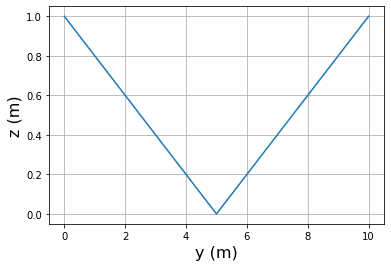
\includegraphics[width=1 \textwidth]{sezionetri.png}
    \caption{Sezione triangolare}
    \label{fig:triangolare_sezione}
\end{minipage}
\ \hspace{2mm} \hspace{3mm} \
\begin{minipage}[b]{8.5cm}
    \centering
    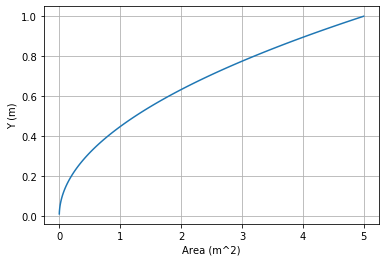
\includegraphics[width=1 \textwidth]{rapporto area altezzatri.png}
    \caption{Rapporto area/altezza}
    \label{fig:triangolare_area/altezza}
\end{minipage}
\end{figure}

\noindent L’andamento dei coefficienti di ragguaglio $\alpha$ e $\beta$ ha comportamenti differenti in base al metodo di calcolo utilizzato: con il metodo dei trapezi i valori oscillano ampiamente per tiranti bassi e si stabilizzano attorno ad un valore costante all’aumentare dell’altezza della superficie libera, mentre con il metodo di Gauss il risultato è costante anche per bassi valori di tirante. 

\begin{figure}[H]
\begin{minipage}[b]{8.5cm}
\centering
    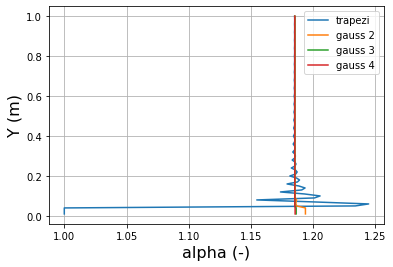
\includegraphics[width=1 \textwidth]{alphatri.png}
    \caption{Andamento coefficiente $\alpha$}
    \label{fig:triangolare_alfa}
\end{minipage}
\ \hspace{2mm} \hspace{3mm} \
\begin{minipage}[b]{8.5cm}
    \centering
    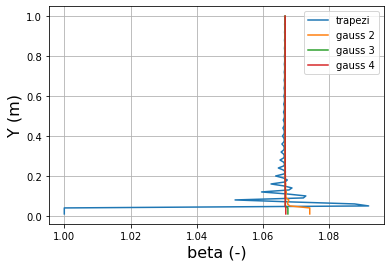
\includegraphics[width=1 \textwidth]{betatri.png}
    \caption{Andamento coefficiente $\beta$}
    \label{fig:triangolare_beta}
\end{minipage}
\end{figure}

\newpage

\noindent La scala di deflusso descritta dal grafico risulta appartenente a un moto uniforme a corrente lenta. 

\begin{figure}[H]
    \centering
    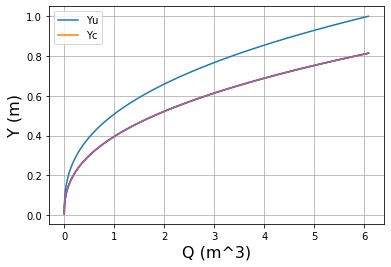
\includegraphics[scale=0.8]{deflussotri.png}
    \caption{Scala di deflusso per una sezione triangolare}
    \label{fig:triangolare_scala_deflusso}
\end{figure}


\subsection{Sezione rettangolare}

\noindent La sezione di seguito analizzata presenta una generica forma rettangolare.
Il rapporto tra l’area della sezione bagnata e l’altezza del tirante risulta lineare per qualsiasi valore assunto.

\begin{figure}[H]
\begin{minipage}[b]{8.5cm}
\centering
    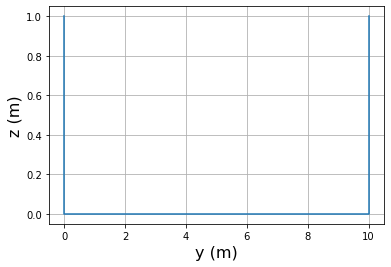
\includegraphics[width=1 \textwidth]{sezioneret.png}
    \caption{Sezione rettangolare}
    \label{fig:rettangolare_sezione} 
\end{minipage}
\ \hspace{2mm} \hspace{3mm} \
\begin{minipage}[b]{8.5cm}
    \centering
    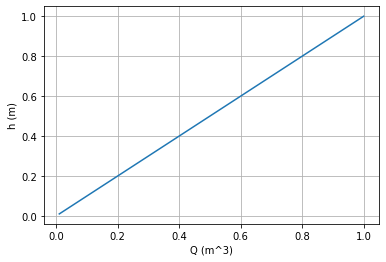
\includegraphics[width=1 \textwidth]{rapporto portata altezzaret.png}
    \caption{Rapporto portata/altezza}
    \label{fig:rettangolare_portata/altezza}
\end{minipage}
\end{figure}

\noindent La regolarità della geometria della sezione si rispecchia nell’andamento dei coefficienti di ragguaglio $\alpha$ e $\beta$, i quali sono costantemente nulli all’aumentare della quota del pelo libero.

\begin{figure}[H]
\begin{minipage}[b]{8.5cm}
\centering
    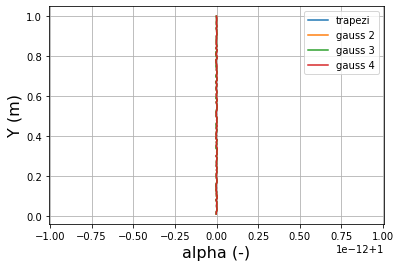
\includegraphics[width=1 \textwidth]{alpharet.png}
    \caption{Andamento coefficiente $\alpha$}
    \label{fig:rettangolare_alfa}
\end{minipage}
\ \hspace{2mm} \hspace{3mm} \
\begin{minipage}[b]{8.5cm}
    \centering
    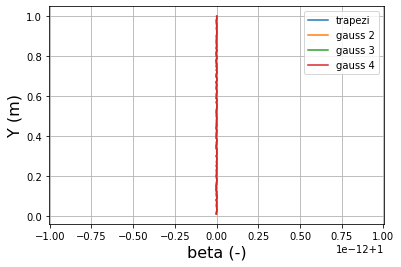
\includegraphics[width=1 \textwidth]{betaret.png}
    \caption{Andamento coefficiente $\beta$}
    \label{fig:rettangolare_beta}
\end{minipage}
\end{figure}

\noindent La scala di deflusso caratteristica di un canale rettangolare riporta l'andamento tipico di un alveo fluviale.

\begin{figure}[H]
    \centering
    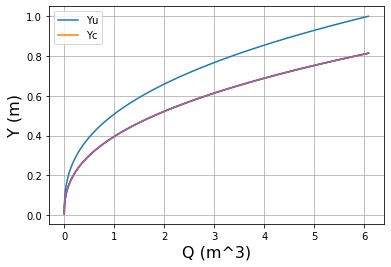
\includegraphics[scale=0.8]{deflussotri.png}
    \caption{Scala di deflusso per una sezione rettangolare}
    \label{fig:rettangolare_scala_deflusso}
\end{figure}

\subsection{1° sezione reale: Adige}
\noindent La sezione presa in esame nel caso attuale appartiene al secondo fiume più lungo in Italia, l’Adige, il quale presenta un alveo fortemente antropizzato, più volte soggetto ad opere di sistemazione fluviale. 
L’asta fluviale che solca la Val d’Adige è stata deviata e regolarizzata in numerosi tratti per permettere lo sfruttamento intensivo del terreno, soprattutto a scopo agricolo. 
Dal grafico, infatti, si può notare una certa regolarità lungo la coordinata trasversale nella forma della sezione, tipica di un letto antropizzato. Il rapporto tra l’area bagnata e il tirante appare leggermente logaritmico, a conferma del fatto che la forma della sezione risulta essere intermedia tra una triangolare e una rettangolare.

\begin{figure}[H]
\begin{minipage}[b]{8.5cm}
\centering
    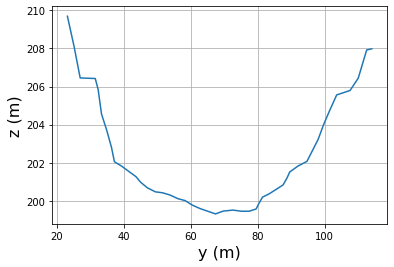
\includegraphics[width=1 \textwidth]{sezioneadi.png}
    \caption{Sezione Adige}
    \label{fig:Adige_sezione}
\end{minipage}
\ \hspace{2mm} \hspace{3mm} \
\begin{minipage}[b]{8.5cm}
    \centering
    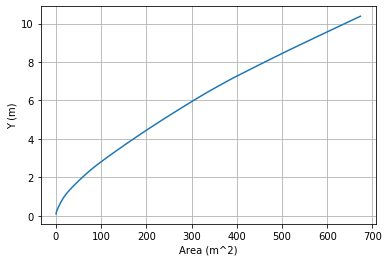
\includegraphics[width=1 \textwidth]{rapporto area altezzaadi.png}
    \caption{Rapporto area/altezza}
    \label{fig:Adige_area/altezza}
\end{minipage}
\end{figure}

\noindent La regolarità della sezione proposta trova riscontro anche nell’andamento simile dei coefficienti di ragguaglio $\alpha$ e $\beta$ al variare del pelo libero. A bassi valori di tirante corrispondono coefficienti con alta variabilità all’interno di un range numerico limitato, i quali però tendono a stabilizzarsi attorno a un valore costante all’aumentare della quota di pelo libero.

\begin{figure}[H]
\begin{minipage}[b]{8.5cm}
\centering
    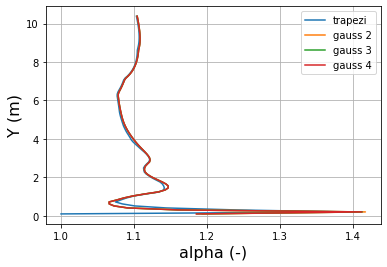
\includegraphics[width=1 \textwidth]{alphaadi.png}
    \caption{Andamento coefficiente $\alpha$}
    \label{fig:Adige_alfa}
\end{minipage}
\ \hspace{2mm} \hspace{3mm} \
\begin{minipage}[b]{8.5cm}
    \centering
    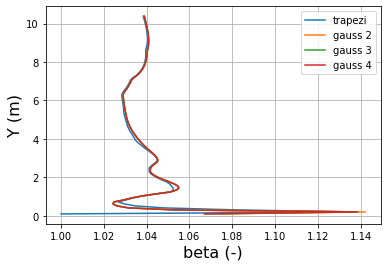
\includegraphics[width=1 \textwidth]{betaadi.png}
    \caption{Andamento coefficiente $\beta$}
    \label{fig:Adige_beta}
\end{minipage}
\end{figure}

\begin{figure} [H]
    \centering
    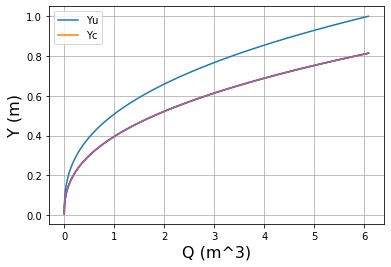
\includegraphics[scale=0.8]{deflussotri.png}
    \caption{Scala di deflusso dell'Adige}
    \label{fig:Adige_scala_deflusso}
\end{figure}

\subsection{2° sezione reale: Tanaro}

\noindent A differenza del caso precedente, la sezione di seguito analizzata appartiene al fiume Tanaro, corso d’acqua tra i maggiori in termini di rilevanza a livello nazionale, caratterizzato da uno sviluppo nel territorio non regolarizzato da opere antropiche.
L’estensione e l’irregolarità dell’alveo del fiume si notano chiaramente dal grafico, dove elemento rilevante per l’analisi di portata della sezione risulta essere lo scavo generatosi sul fondo del corso d’acqua. Tale particolarità altera l’andamento ipoteticamente lineare del rapporto tra area bagnata e tirante, di fatto dividendolo in due tratti con coefficiente angolare diverso: il primo tratto, più ripido, legato al riempimento della fossa, e il secondo, meno ripido, legato al riempimento totale dell’alveo.

\begin{figure}[H]
\begin{minipage}[b]{8.5cm}
\centering
    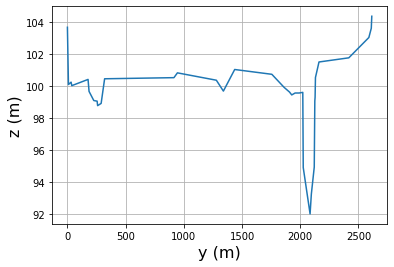
\includegraphics[width=1 \textwidth]{sezioneta.png}
    \caption{Sezione Tanaro}
    \label{fig:Tanaro_sezione}
\end{minipage}
\ \hspace{2mm} \hspace{3mm} \
\begin{minipage}[b]{8.5cm}
    \centering
    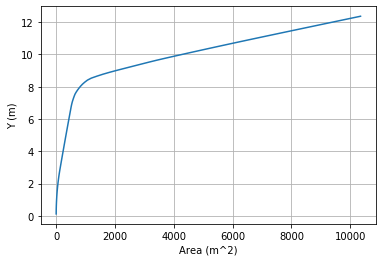
\includegraphics[width=1 \textwidth]{rapporto area altezzata.png}
    \caption{Rapporto area/altezza}
    \label{fig:Tanaro_area/altezza}
\end{minipage}
\end{figure}

\noindent I coefficienti di ragguaglio seguono un andamento influenzato dal medesimo elemento: una convergenza dei parametri attorno ad un valore costante nella zona dello scavo, seguita da un brusco aumento leggermente contenuto soltanto nel tratto di riempimento finale.

\begin{figure}[H]
\begin{minipage}[b]{8.5cm}
\centering
    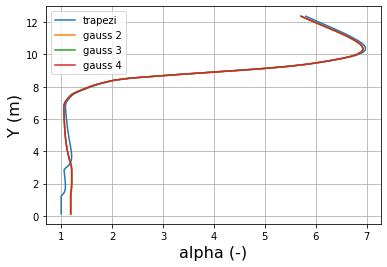
\includegraphics[width=1 \textwidth]{alphata.png}
    \caption{Andamento coefficiente $\alpha$}
    \label{fig:Tanaro_alfa}
\end{minipage}
\ \hspace{2mm} \hspace{3mm} \
\begin{minipage}[b]{8.5cm}
    \centering
    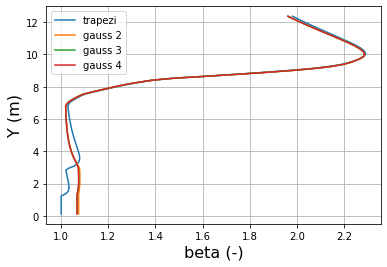
\includegraphics[width=1 \textwidth]{betata.png}
    \caption{Andamento coefficiente $\beta$}
    \label{fig:Tanaro_beta}
\end{minipage}
\end{figure}

\noindent Anche la scala di deflusso del fiume risente della peculiare forma dell’alveo, presentando un tratto iniziale di rapido innalzamento del pelo libero seguito da un tratto di curva più dolce nel momento in cui il riempimento interessa la totalità della sezione. Il confronto tra la scala di deflusso critica e quella analitica ci consente di distinguere due diversi comportamenti della corrente: un carattere fluviale in corrispondenza dello scavo sostituito da un carattere torrentizio nel resto dell’alveo.

\begin{figure}[H]
    \centering
    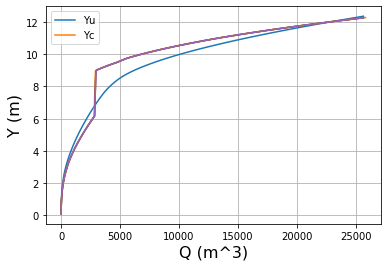
\includegraphics[scale=0.8]{deflussota.png}
    \caption{Scala di deflusso del Tanaro}
    \label{fig:Tanaro_scala_deflusso}
\end{figure}


\subsection{3° sezione reale: Vara}

\noindent La terza sezione analizzata appartiene al fiume Vara, il maggior corso d’acqua della Liguria.
La forma della sezione presenta un contorno fortemente irregolare, caratterizzato da piccoli avvallamenti e sponde di lunghezza irregolare.

\begin{figure}[H]
\begin{minipage}[b]{8.5cm}
\centering
    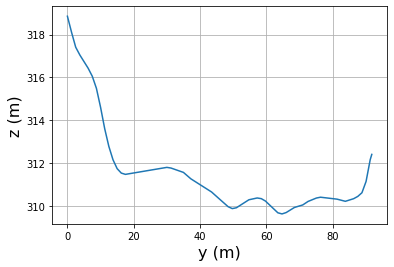
\includegraphics[width=1 \textwidth]{sezioneva.png}
    \caption{Sezione Vara}
    \label{fig:Vara_sezione}
\end{minipage}
\ \hspace{2mm} \hspace{3mm} \
\begin{minipage}[b]{8.5cm}
    \centering
    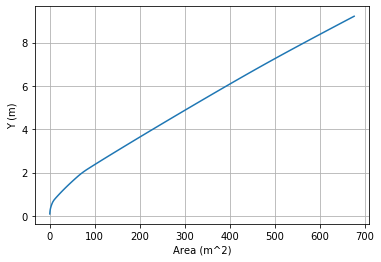
\includegraphics[width=1 \textwidth]{rapporto area altezzava.png}
    \caption{Rapporto area/altezza}
    \label{fig:Vara_area/altezza}
\end{minipage}
\end{figure}

\noindent I coefficienti di ragguaglio $\alpha$ e $\beta$ assumono valori irregolari per tirante basso sia con il metodo di Gauss che con il metodo dei trapezi, salvo poi stabilizzarsi in entrambi i casi una volta raggiunti i massimi valori di tirante.

\begin{figure}[H]
\begin{minipage}[b]{8.5cm}
\centering
    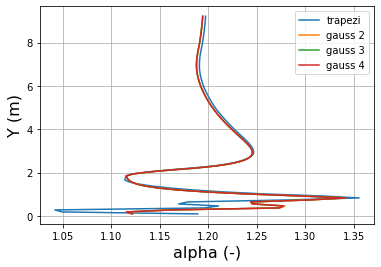
\includegraphics[width=1 \textwidth]{alphava.png}
    \caption{Andamento coefficiente $\alpha$}
    \label{fig:Vara_alfa}
\end{minipage}
\ \hspace{2mm} \hspace{3mm} \
\begin{minipage}[b]{8.5cm}
    \centering
    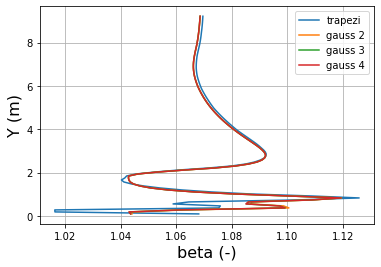
\includegraphics[width=1 \textwidth]{betava.png}
    \caption{Andamento coefficiente $\beta$}
    \label{fig:Vara_beta}
\end{minipage}
\end{figure}

\noindent Dalla scala di deflusso si può riscontrare il comportamento fluviale assunto dalla corrente del corso d’acqua, anche se con un divario tra tirante uniforme e tirante critico meno marcato rispetto ai fiumi di pianura.

\begin{figure} [H]
    \centering
    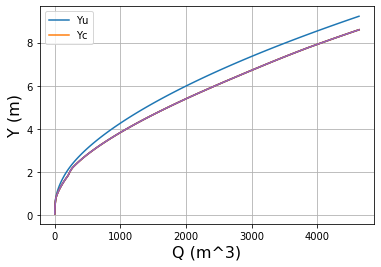
\includegraphics[scale=0.8]{deflussova.png}
    \caption{Scala di deflusso del Vara}
    \label{fig:Vara_scala_deflusso}
\end{figure}

\newpage

\begin{thebibliography}{}
\bibitem{Collischonn, W. 2013}
Collischonn, W. (2013) \textit{Hidrologia para engenharia e ciências ambientais}. ABRH, Porto Alegre
\bibitem{Adami, L. 2019}
Adami, L. (2019) \textit{Dispense del corso di Idrodinamica (a. a. 2019/2020)}.
\bibitem{Quarteroni A. 2014}
Quarteroni A., Sacco R., Saleri F., Gervasio P. (2014) \textit{Matematica Numerica}. Springer, Milano
\end{thebibliography}

\end{document}